\documentclass[acmsmall]{acmart}

\usepackage{graphicx}
\usepackage{tikz}
\usetikzlibrary{arrows}
\usepackage{verbatim}
%\usepackage{algorithm}
%\usepackage[noend]{algpseudocode}
%\usepackage{amssymb}
%\usepackage{amsfonts}
%\usepackage{amsmath}
%\let\proof\relax\let\endproof\relax
%\usepackage{amsthm}
% \usepackage{graphicx}
%\usepackage[all]{xy}
\usepackage{array}
\usepackage{enumitem}
%\usepackage{cite}
\usepackage{natbib}
\usepackage{wrapfig}
\usepackage{algorithm}
\usepackage{algpseudocode}
\theoremstyle{definition}
\renewcommand{\qedsymbol}{\hfill\ensuremath{\blacksquare}}
%\newtheorem{definition}{Definition}[section]
% If you use the hyperref package, please uncomment the following line
% to display URLs in blue roman font according to Springer's eBook style:
% \renewcommand\UrlFont{\color{blue}\rmfamily}
%\usepackage[breaklinks=true]{hyperref}
\usepackage{hyperref}
%\usepackage{breakcites}
%\renewcommand\UrlFont{\color{blue}\rmfamily}
\newcommand{\secref}[1]{Section \ref{#1}: \nameref{#1}}

\usepackage{multicol}
\keywords{Attestation, Trust, Verification}
\begin{CCSXML}
<ccs2012>
   <concept>
       <concept_id>10002978.10002986.10002987</concept_id>
       <concept_desc>Security and privacy~Trust frameworks</concept_desc>
       <concept_significance>300</concept_significance>
       </concept>
 </ccs2012>
\end{CCSXML}

\ccsdesc[300]{Security and privacy~Trust frameworks}

\newcommand{\defn}[2]{
  \begin{flushleft}
  \begin{definition}[\textbf{#1}]\label{defn:#1}
    #2
  \end{definition}
  \end{flushleft}
}

\begin{document}
%
\title{Attestation: A Taxonomy and Evaluation}
%
%\titlerunning{Abbreviated paper title}
% If the paper title is too long for the running head, you can set
% an abbreviated paper title here
%
%
\author[W. Thomas]{Will Thomas}
\affiliation{%
  \institution{The University of Kansas}
  \department{Institute for Information Sciences}
  \streetaddress{2335 Irving Hill Rd}
  \city{Lawrence}
  \state{KS}
  \postcode{66045}
  \country{USA}}
\email{30wthomas@ku.edu}
%
\begin{abstract}
  %% 1. State the problem
  %% 2. Say why it’s an interesting problem
  %% 3. Say what your solution achieves
  %% 4. Say what follows from your solution
  Remote attestation is a method through which
  principals may exchange information in order
  to establish trust. Many varying methods
  for achieving this goal have been proposed and explored,
  and the applications of attestation are extremely far reaching.
  For this reason, diverging nomenclature has appeared, along
  with a general lack of an overall attestation view across
  the many sub-classifications of attestation.
  In this review, we will attempt to unify the nomenclature used
  for attestation, as well as establish a general taxonomy for attestation
  methods. Further, we will summarize the prominent current
  methods for attestation and review the strengths and
  weaknesses of each, while exploring typical attestation use cases.
\end{abstract}

\maketitle              % typeset the header of the contribution
%
%
%
\section{Introduction}

In this paper, we will attempt to set-up a general framework for
describing and categorizing attestation, as well as a more in-depth
exploration of the benefits and limitations of the specific attestations paradigms.
In order to achieve this goal, we must start with some common definitions necessary
to describe nearly all attestation scenarios.

\defn{Attestation}{
  \textbf{Attestation} is the process of producing a verifiable report of evidence from a system
  as presented by \citet{Sadeghi:04:Property-based-, Haldar:04:Semantic-Remote,Coker::Principles-of-R}.

  The primary motivation behind attestation is not as a
  malware preventive measure\footnote{as \citet{Loscocco:98:The-Inevitabili} established perfect prevention is impossible}, 
  but rather a detection method to allow for the revocation of trust
  from a corrupted principal.
}

\begin{figure}[ht]
  \centering
  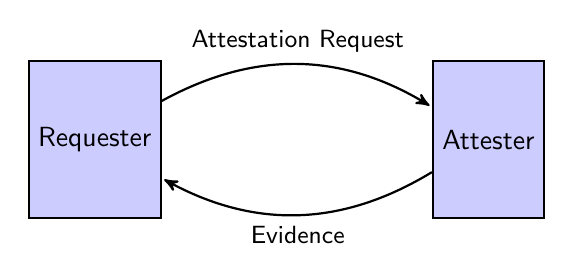
\begin{tikzpicture}[->,>=stealth',shorten >=1pt,auto,node distance=2.0cm,
    thick,main node/.style={rectangle,fill=blue!20,draw,
        font=\sffamily,minimum height=20mm,minimum width=10mm},
    io node/.style={rectangle,
        font=\sffamily,minimum height=5mm,minimum width=10mm}]

  \node[main node] (NM) {Requester};
  \node[main node] (NME) [node distance=5.0cm, right of=NM] {Attester};

  \path[every node/.style={font=\sffamily\small, fill=white,inner sep=1pt}]
  (NM) edge [bend left=30] node[above=1mm] {Attestation Request} (NME)
  (NME) edge [bend left=30] node[below=1mm] {Evidence} (NM)
  ;
\end{tikzpicture}

%%% Local Variables: 
%%% mode: latex
%%% TeX-master: "csur23"
%%% End:

  \caption{Remote attestation.}
  \label{fig:remote-attestation}
  \Description{Remote Attestation Figure}
\end{figure}

Attestation has additionally been referred to as ``semantic remote attestation'',
which represents that the process of attestation will involve two main (typically separate/remote) principals that exchange
evidence regarding the semantics/behaviors of the system, ultimately to establish trust in
the faithful execution of some semantics by a certain principal (the \nameref{defn:Attester}):

\defn{Attestation Request}{
  The Attestation Request (Fig~\ref{fig:remote-attestation}) is a request made from the Requester to the Attester asking for attestation to
  take place. The Attester then returns evidence to the Requester.
}

\defn{Requester}{
  The \textbf{Requester} is the principal that sends Attestation Request's to some Attester.

  The Requester will also have some method of validating/verifying that the returned Evidence
  from the Attestation Request is valid. For this reason, the Requester is also on occassion referred to
  as the \textbf{Verifier} or \textbf{Appraiser}.
}

\defn{Attester}{
  The \textbf{Attester} is the principal that will receive Attestation Request's from a Requester,
  process them, and return evidence to the Requester.

  Other word frequently used to refer to this principal are: \textbf{Prover} and occassionally \textbf{Target}.
  The usage of \textbf{Target} is only appropriate when the Attester is itself the target of an Attestation
  Request, and not just a servicing principal that performs \textbf{Measurement} on some other entity.
}

Although in many cases, the Requester will also be the principal that requires evidence about a Target system,
there may be an additional principal involved if the Attestation Request to the Attester is made through a Third Party.
In this case, we need a \textbf{Relying Party}.
\defn{Relying Party}{
  The \textbf{Relying Party} is a principal who wishes to access the evidence report regarding an Attester for
  the purpose of making a \textbf{Trust Decision}.
}

\defn{Trust Decision}{
  \citet{Martin:08:The-ten-page-in} established a group of
  properties that will help establish ``trust'' in an principal.

  These properties are:

  \begin{itemize}
    \item strong identity
    \item composition of ``good'' parts
    \item observation of ``good'' behavior
  \end{itemize}

  The definition of ``good'' must remain ambigious when we
  analyze principals from an abstract level, and the determination of
  ``good'' is left as a problem for measurement and the Attestation
  System Administrator.

  Many times in Attestation however, the nuances of these requirements and the various ways
  to establish trust are quite complicated.
  These properties and ``trust'' in general are explored further in \secref{sec:Attestation-Requirements}
}
% The ``properties'' that are worthy of verification can range
% widely and a strict definition for it is highly context specific.
% Almost universally though, some properties are desirable to know,
% and have been enumerated by 
\subsection{Attestation Types} \label{sec:Attestation-Types}
\begin{figure}[ht]
  \begin{tabular}{| c | c | c || c |}
    \hline
    Relying Party & Requester & Attester & Attestation Type          \\
    \hline \hline
    $X$           & $X$       & $X$      & Self-Attestation/Auditing \\
    $X$           & $X$       & $Y$      & Direct Attestation         \\
    $X$           & $Y$       & $Y$      & Strong Report Attestation \\
    $X$           & $Y$       & $X$      & Third-Party Auditing      \\
    $X$           & $Y$       & $Z$      & Third-Party Attestation   \\
    \hline
  \end{tabular}
  \caption{Table of Attestation Types}
  \label{fig:Attestation-Type-Table}
  \Description{Table labeling the type of remote attestations based on the relationships between the principals involved}
\end{figure}

Depending on the relationships between the Relying Party, Requester, and Attester;
the type of Attestation can change. The 5 main possible relationships are depicted in
Figure~\ref{fig:Attestation-Type-Table}, where $X,Y,Z$ represent different
principals in an attestation.

Note that an obvious extension to these types would involve when the Attester and Target are not one and the same.
This case usually would be considered a form of \nameref{defn:Delegated Attestation},
but more nuance may apply. Extending this classification is left to future work.

\subsubsection{Self-Attestation/Auditing}
In \textbf{Self-Attestation/Auditing}, the same principal is the Relying Party, Requester, and Attester. This
represents a special case of Attestation that is not remote at all.
In Self-Attestation, evidence is produced by the principal as a means to verify to itself or a possible end-user
that the system is not compromised.

This form of attestation in practice is typically not recognized as attestation and would best be compared to a
form of malware detection or anti-virus software that runs on a computer.

\subsubsection{Direct Attestation}
In \textbf{Direct Attestation}, the Relying Party and the Requester are the same principal, and the Attester is
separate. This is a typical attestation use-case where the Relying Party has the ability to Appraise/Verify
the Attestation Evidence returned by the Attester.

\subsubsection{Strong Report Attestation}
% TODO: Is this real
\textbf{Strong Report Attestation} is a type of Attestation where a Trusted Component of the
single principal comprising the Requester and Attester is able to gather evidence as to that
principals state, reliably verify that evidence, and serve reports to any Relying Party.

This type of Attestation is in practice very difficult to realize as having a high-level Trusted
Component of a principal that can both gather and verify evidence securely
is difficult to construct.

\subsubsection{Third-Party Auditing}
\textbf{Third-Party Auditing} is very similar to Self-Attestation, except the Verification of
the evidence the principal gathers is left to a Third-Party entity rather than itself.

This is another conceivable method where the actual attestation process is very similar to a
malware detection process that utilizes a Third-Party database to identify
adversary actions.

\subsubsection{Third-Party Attestation}
In \textbf{Third-Party Attestation}, all principals are distinct. However, a certain level of implicit trust
must exist between the Relying Party and the Requester to believe that the report the Requester generates for
consumption by the Relying Party is a faithful representation of the state of the evidence provided by the Attester.
This implicit trust can be resolved to some extent by layering attestation protocols (\secref{sec:Layered-Attestation}).

Third-Party Attestation is very similar to Direct Attestation, except for the Relying Party either lacks the ability
to Appraise evidence provided by the Attester, or the Attester does not trust the Relying Party with its evidence, but
will trust the Requester to Appraise it.

Ultimately, this is one of the most flexible types of attestation, and any general purpose attestation protocol must
support Third-Party Attestation.


\section{Classification}

There are two main classes of Attestations: \textbf{Software} and \textbf{Hardware}, along with an additional \textbf{Hybrid} sub-class.
The primary distinquishing difference between these two classes is
the existence/utilization of a \nameref{defn:Trusted Hardware Component}.

\begin{figure}[ht]
  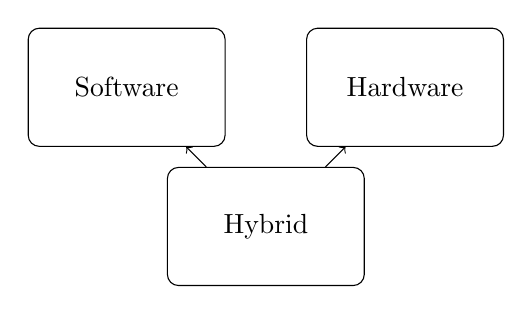
\begin{tikzpicture}[
      node distance=2.5cm,
      main node/.style={draw, rounded corners, align=center, minimum width=2.5cm, minimum height=1.5cm}
    ]
    % Top classes
    \node (hybrid) [main node, align=center] {Hybrid};
    \node (software) [main node, above left of=hybrid] {Software};
    \node (hardware) [main node, above right of=hybrid] {Hardware};

    % Hybrid class inheriting from Software and Hardware
    \draw[->] (hybrid) -- (software);
    \draw[->] (hybrid) -- (hardware);
  \end{tikzpicture}
  \label{fig:Attestation-Classes}
  \caption{Attestation Class hierarchy}
  \Description{A hierarchy of attestation classes showing that software and hybrid are top level classes, and hybrid inherits from both}
\end{figure}

\defn{Trusted Hardware Component}{
  A hardware component (that is implicitly trusted to have been constructed correctly) that provides the following functions:
  \begin{enumerate}
    \item A secure hardware private key
    \item A secure random number generator
    \item Tamper resistant memory storage
    \item Cryptographic functions
  \end{enumerate}
}
The \citet{Trusted-Computing-Group:07:TCG-TPM-Specifi} in their specification for the Trusted Platform Module (TPM), include all these features.

\subsection{Hardware Attestation}
This class of attestation is is characterized by its requirement for a \nameref{defn:Trusted Hardware Component}
to establish a Hardware Root of Trust (RoT). This Root of Trust will utilize the tamper resistant
memory storage to store attestation evidence, and then sign it with the secure hardware private key,
and the provided cryptography functions. This ensures that this tamper-proof
hardware component will capture evidence of any malicious actions and not be erasable without
corrupting a presumed uncorruptible component of the system.

Hardware Attestation also proposes that the Root of Trust be used as a base from
which additional trust decisions can be made moving up to a final Binary/Property/Behavior/etc.
of a principal. This Chain of Trust concept interplays well with \nameref{sec:Layered-Attestation} 
presented later.

Hardware Attestation has proven particularly relevant to \nameref{defn:Binary Based Attestation} as the
tamper resistant memory storage of a Trusted Hardware Component provides a secure location to store
evidence regarding a binary that cannot be erased by transient malware.
Additionally, tamper resistant memory storage such as the Program Control Registers (PCRs) of the
TPM can be used to verify secure boot occurs.
A common extension to the definition of Trusted Hardware Component requires that boot is either
securely completed, or boot evidence is recorded within the Trusted Hardware Component to be
verified later.

\citet{Kuhn:07:Realizing-prope} demonstrated how a TPM can be used as a hardware root of trust.
Using just a Trusted Computing Group (TCG) trusted hardware component (such as the TPM)
a viable hardware based attestation system can be built, without other OS modifications.

\subsection{Software Attestation}
% TODO: Hunt down some good early articles on this
Software based attestation is a class of attestation that is useful for incorporating into legacy systems,
or utilizing in cases where the ability for hardware support is limited
(such as low-power embedded devices, IoT, etc.).
Software based attestation has three main components:
\begin{enumerate}
  \item Does not require specialized hardware to complete attestation requests.

        If specialized hardware is required for an attestation mechanism, it should be classified as hardware based attestation
  \item Relies on the timeliness of attestation request responses to establish trust in the attestation evidence.

        This is implemented through a requirement that a specific, constant, amount of computational and memory resources (typically 100\%) will be allocated to serving the attestation request as soon as the attester receives it. Thus the time for the attestation request to be served should be relatively constant as well.
        The verifer/requester should have an understanding of the expected time it will take for an attestation request to be served, and invalidate any evidence/responses that are returned after a time longer than the attestation should've taken.

        This helps thwart spoofing attacks where an adversary could utilize a cloned, uncorrupted version of the system they have taken over to generate good evidence in response to attestation requests. The issue of spoofing attacks is solved in hardware based attestation through the hardware root of trust signing attestation evidence; essentially the uncloneable secret key is used.

        In order for spoofing attacks to take place in software based attestation, the adversary must be able to dispatch any attestation request to its uncorrupted ``exemplar'' system and respond with the evidence from that system just as quickly as it would take for it to do the attestation evidence gathering and computation on itself in real-time.
        This is generally considered to be highly improbably and thus trust in the attestation evidence is merited should it be returned in a timely fashion.

  \item Requires a direct communication method between the attester/prover and requester/verifer.

        % TODO: Look for the alternatives
        This requirement (although some research has proposed possible alternatives)
        is primarily enforced by requirement (2).
        The unreliability of a multiple hop/indirect communication method would make trusting
        software based attestation results too difficult, so it is generally considered required that direct communication be established.
\end{enumerate}
\citet{Armknecht:2013:Software-Attestation-Framework} presents a strong background on software based attestation systems, demonstrating the inherent strengths in that it can be easily applied in many areas. The great weakness of software attestation schemes lies in the (typical) requirement of the software attestion service to hijack all computing and memory resources of the prover/attester to ensure the timely return of evidence to a relying party/verifier. This is because software attestation implicitly relies on a timing argument for it to be considered secure.
The returned evidence package must be received within a certain time constraint, that is generally considered infeasible for an adversary to have falsified.

One great limitation of software based attestation is that it
suffers from the Time-of-Check-Time-of-Use (TOCTOU) problem. Transient malware with the ability to erase itself poses a great problem for Software Attestation as without a hardware root of trust to track and preserve any record of malware interference, software attestation may return ``good'' evidence due to an inability to detect the malware that has erased its presence. \citet{nunes2019vrased,Nunes:2021:TOCTOU-Remote-Attestation} all explore the primary issues of Software Attestation and propose solutions to the TOCTOU problem and
dealing with a transient adversary.

A particular vulnerability of Software based attestation is Computation Denial of Service (CDoS).
\citet{Bampatsikos:2019:BARRETT} propose using a Public Ethereum Network (PEN) to solve the CDoS vulnerability of software based attestation systems. As previous mentioned, software based attestation approaches require an extremely timely computation and return of the attestation evidence in order for the evidence to be verified and approved. This is typically achieved through shunting all computational and memory resources of the prover/attester towards the attestation request.
This opens up software based attestation to an obvious DoS vulnerability if attestation requests are repeatedly made.
The solution proposed by \citet{Bampatsikos:2019:BARRETT} with their system BARRETT is a PEN for which cryptocurrency must be mined for each attestation request, otherwise they will be dropped without any attestation evidence gathering or computation taking place.
This is stronger than a nonce or timestamp approach that may thwart some, but not all CDoS attacks.

\subsection{Hybrid Attestation}
Hybrid attestation, as one might expect, combines features of both hardware based and software based attestation.
Rather than the strict requirement that hardware not be utilized in the attestation process, some specific (likely trusted)
hardware component will be used in hybrid attestation.
However, this hardware component will not reach the level of complexity, trust, or power that the \nameref{defn:Trusted Hardware Component}
provides, or a pure hardware based attestation solution would be better.
Some examples of hybrid based attestation systems have been assembled here:

\begin{itemize}
  \item \citet{Javaid:2020:Defining-Trust-IoT-Blockchain-Attestation} particularly utilized Physical Unclonable Functions (PUF) as a mechanism for hybrid attestation measurement; requring hardware support for PUFs, but software mechanism for verifying the integrity of the results. They additionally make use of a Blockchain as an attestation entity registration/identification system.
        The use of a blockchain as an identification server for attestation systems is a common theme that falls into the realm of \textbf{Explicit Identity Management} (similarly to a central \textbf{Certificate Authority} or other \textbf{Trusted Third Party}).

  \item Further hybrid attestation work is explored by \citet{Mondal:2023:PReFeR-Attestation-Protocol} in there system PReFeR, where instead of utilizing PUF's, Physically Related Functions (PRF's) are used. PRF's do not require hardware support for secure storage, and also will not require computationally intensive crypto operations. Since this is a hybrid attestation scheme, the timeliness of a response is critical for validating its integrity. These means that the computational intensivity of the attestation measurements matters a lot for performance reasons. Reducing the amount of computation that must occur dynamically through Hardware Performance Counters (HPCs) is a key feature of the PReFeR work that keeps it a hybrid solution requiring some hardware support, but mitigating many limitations of software attestation such as TOCTOU.
        Ultimately, PRF's also allow for easy non-Binary attestation methodologies, as PUF's will need a large database of possible acceptable Binary attestation results for verification, where as PRF's will not.

\end{itemize}

\section{Attestation Methods}
In this section we will explore some of the general methodologies used by attestation systems.
These methodologies are a characterization of the measurement target that the attestation is
being performed on. Differing methodologies offer different advantages: some
are much easier to implement, but harder to verify; others have much more complex
measurement processes, but offer greater flexibility when it comes to making trust decisions.

\defn{Binary Based Attestation}{
  \textbf{Binary Based Attestation} was the first, and most obvious, attestation method.
  Using a simple comparison between the hash of a running program binary, and comparing it to a
  ``golden value'' that the binary should have, you can tell if the running binary is the
  expected binary. Many of the early attestation definitions and systems (\citet{Brickell:04:Direct-anonymou, ietf2023rats,Gu:2008:Remote-Attestation-on-Program-Execution})
  implemented binary attestation.

  Despite the robustness of Binary Attestation, it is severely limited when viewed
  in light of modern constantly evolving and changing systems.
  Binary Attestation has one acceptable ``golden value'' that will be considered
  ``good'' during the appraisal/verification process. This limitation is addressed
  by the many alternative attestation methods that have been proposed following Binary Attestation.
}

\defn{Direct Anonymous Attestation (DAA)}{
  \textbf{Direct Anonymous Attestation (DAA)} is a method of \textbf{Binary, Hardware Attestation} first introduced by \citet{Brickell:04:Direct-anonymou} that specifically upholds the principle of anonymity.
  A \textbf{Trusted Execution Environment (TEE)} is established with the use of a \textbf{Trusted Platform Module (TPM)} (or extensibly any other \nameref{defn:Trusted Hardware Component}).
  The TPM has a specific \textbf{Attestation Identity Key (AIK)} that can be verified through the use of a \textbf{Trusted Third Party (TTP)} that acts as a \textbf{Certificate Authority (CA)}.
  This form of attestation has extremely niche use cases, and manages to present Attestation Reports to Relying Partys
  allowing make trust decisions without disclosing the identity of the Attester.
}

\defn{Privilege-Based Attestation}{
  \citet{Rauter:2015:Privilege-Based-Remote-Attestation} propose PRIBA (PRivilege-Based remote Attestation) as an extension of binary attestation. One of the great limitations of binary attestation is that knowledge of all possible ``good'' configurations of an attestation target/attester is extremely difficult.
  Instead, the good configurations of the attester are established through binary analysis of the end executable to be attested to. This executable is analyzed to
  determine ``modules'' that it depends on, in the form of system call APIs. These modules are then themselves attested to for their possible good configurations.
  If a binary utilizes modules that are themselves attested to and shown to be in a ``good'' state, then the overall binary is considered to be ``good''.
  In this way, PRIBA is an inductive approach to attestation, as the binary needs to be made of good parts to be verified.
  However, it does not quite meet the standards for \secref{sec:Layered-Attestation} that will be explored later.
}

\defn{Property Based Attestation}{
  \textbf{Property based attestation} was introduced by \citet{Sadeghi:04:Property-based-} as a more general model of attestation,
  that would help solve some of the limitations of Binary Attestation.
  Rather than verifying a specific binary is running with specific configurations,
  property based attestation attempts to establish that a certain ``property'' of a system exists.
  For this reason, property based attestation has a wider range of acceptable evidence that will lend
  towards convincing a verifer/requester that the property they are looking to see in the attester actually exists.

  This was further elaborated upon by \citet{Chen:2006:Protocol-Property-Based-Attestation} where they actually designed a general protocol for which property based attestation could occur.

  Some examples of properties we would want to verify about a system are:
  \begin{itemize}
    \item Up to date software
    \item Running virus checker
    \item Kernel Integrity Checks (\citet{Loscocco:07:Linux-kernel-in})
  \end{itemize}
}

\defn{Behavioral/Policy Attestation}{
  Behavioral Attestation was a general high-level method for attestation
  introduced by \citet{Li:2006:Efficient-Attestation-for-Trustworthiness}
  for verifying that a system policy or behavior is being abided by.
}

\defn{Model-Based Behavioral Attestation}{
  This method for attestation is an extension of \nameref{defn:Behavioral/Policy Attestation} introduced by \citet{Alam:2008:Model-Based-Behavioral-Attestation}.
  They utilized Usage Control (UCON) as a model for attester policy, and then gather evidence that the UCON model is not violated.
  Specifically, Model-Based Behavioral Attestation identifies system behaviors and associations between executing processes. They are codified in a low-level policy language and as long as no events violate the provided policy, this is evidence of a ``good'' system.

  Specifically, lack of evidence of events violating the model implies a ``good'' attester.
}

\defn{Delegated Attestation}{
  Delegated Attestation is a hybrid attestation method introduced by \citet{Ammar:2021:Delegated-Attestation} which involves augmenting an attestation system with a dedicated piece of attestation hardware. While each attester itself will not require specialized hardware support, their software will be modified to transmit all events to this dedicated ``Attestation Proxy'' that will manage attestation evidence securely.

  This approach particularly thwarts TOCTOU issues that arise in software based attestation systems by adding the specialized hardware based attestation system. Transient malware will be recorded by the trusted hardware components of the Attestation Proxy and cannot be erased, even if the malware erases traces of itself from the original attester.
}

\subsection{Attestation Timings}
\label{sec:Attestation-Timings}
There are two main types of Attestation Timings:
\begin{enumerate}
  \item On-Demand:

        The Attestation Request is serviced once it arrives and fresh evidence is gather at the time of attestation servicing

  \item Periodic:

        This is typically completed with some form of self-measurement and attestation results caching. Particularly, attestation evidence is gather occassionally and stored in the memory of the attester. This evidence is then returned to the requester when an attestation request arrives.

\end{enumerate}

\subsection{Attestation Patterns} \label{sec:Attestation-Patterns}

\subsubsection{Layered Attestation} \label{sec:Layered-Attestation}

\textbf{Layered Attestation} is a general pattern for attestation that involves Attestation Service Providers (ASPs)
that can execute either arbitrary measurements, or further attestation protocols themselves.
The expressive power of ASPs is the key feature of layered attestation, as an the same attestation
protocol may act differently depending on the target of its attestation.

It is worth noting that ASPs are not non-deterministic\footnote{Although nothing
  but the Appraisal/Verification process most likely necessitating determinicity would forbid it},
but that they may take variable arguments based upon the target of attestation that
will describe a targets structure; allowing for an inductive approach to
be taken by all ASPs.

\citet{helble2021flexible} introduce a set of general patterns that attestation requests will likely take and establish the security benefits and limitations of each approach. These mechanisms all utilize layered attestation,
and are themselves meant to be layered upon one another to create more complex attestation protocols.

In the same realm of property based attestation, Domain Specific Languages for attestation have been developed to help create attestation protocols that can achieve fine-grained selection of properties you wish to verify. Specifically, the
\citet{copland-lang} developed Copland, a DSL meant for attestation,
along with an accompanying verified Attestation Manager (\citet{copland-avm-github}).
Attestation DSL's allow for specific Attestation Service Providers (ASPs) to represent a measurement of a
specific property.

\citet{petz2022innovations} design and verify a Attestation Virtual Machine, as a running executable which can consume Attestation Requests in the form of Copland protocols.

Further, they demonstrate how the assumptions necessary for securely gathered attestation evidence
via an Attestation Manager or Virtual Machine can be satisfied with a strict process isolation mechanism, such as the seL4 microkernel (\citet{Klein:09:seL4:-formal-ve}).

\subsubsection{Swarm Attestation} \label{sec:Swarm-Attestation}
Swarm attestation is an attestation pattern that will utilize many attesters
in a parallel fashion to efficiently make trust decisions. \citet{ kuang2019esdra,carpent2017lightweight,Wedaj:2019:DDA:3328797.3325822}
all explore using swarm attestation to efficiently attest to a
large number of attesters with a single protocol.

\begin{flushleft}

  The key characteristics of swarm attestation are:
  \begin{itemize}
    \item Multiple Attesters
    \item A propagating attestation request across all Attesters in the swarm
    \item A protocol that is more efficient to operate in parallel rather than individually.
  \end{itemize}

  Additionally, a swarm attestation will typically have a
  non-standard network topology where the connection
  between the Requester and Attesters does not necessarily
  need to be direct. If all Attesters are directly connected
  to the Requester, it may be better characterized as
  \textbf{Distributed Attestation}.
\end{flushleft}

\section{Attestation Requirements}
\label{sec:Attestation-Requirements}
Now that we have established a taxonomy of attestation, we will
turn our attention towards the evaluation of attestation systems.
In particular, we will review the evolving requirements of attestation
systems that have been devised to secure them and the results they provide.

\subsection{5 Principles of Attestation}
One of the most pivotal works on the requirements for
Remote Attestation was developed my \citet{Coker::Principles-of-R}.
In this work, \citeauthor{Coker::Principles-of-R} outlined 5 principles that attestation frameworks must incorporate:
\begin{enumerate}
  \item (Freshness) Evidence should reflect the system state at the time of evidence gathering

  \item (Comprehensive Information) Attestation should have sufficient access to gather relevant evidence and evidence should provide a comprehensive view of the system.

  \item (Constrained Disclosure) The attester/target should be able to control what information about their system is disclosed and to whom it is disclosed.

  \item (Semantic Explicitness) Evidence should have a well-defined formal semantics to inform the trust judgement that the appraiser/verifier will undertake.

  \item (Trustworthy Mechanism) A fundamental part of trusting attestation evidence results is trusting the attestation infrastructure. Therefore, evidence of the ``good'' construction of the attestation infrastructure should be provided in evidence to the verifier.
\end{enumerate}
The keen reader will notice that we have already presented examples
of attestation frameworks that may abide by these principles but can
still be easily exploited.
One such example would be the case of software binary attestation,
where the evidence reflects the state of a running executable
at exactly measurement time. However, transient malware may be able to
erase evidence of its presence then restore itself before a
security critical operation occurs (the TOCTOU problem).
The attestation system abided by all 5 principles, but still has a glaring vulnerability\footnote{One major factor for this is that the work establishing the 5 Principles operated primarily in the context of hardware based attestation; where the TOCTOU problem is essentially solved by a \nameref{defn:Trusted Hardware Component}}.

\subsection{14 Goals of Attestation}
Given that the 5 Principles are insufficient to prevent
all attacks on attestation protocols, extensions to the principles
were done by \citet{Usman:2023:Attestation-Assurance-Arguments,Banks:2021:Remote-Attestation-Literature-Review} to expand
upon the requirements necessary for securing attestation systems. \\
\citeauthor{Usman:2023:Attestation-Assurance-Arguments} established
14 goals of attestation schemes in \cite{Usman:2023:Attestation-Assurance-Arguments}:
\begin{enumerate}
  \item Acceptably secure remote attestation
  \item Protection of Verifier, Target, and Attestation Agent.
  \item Secure communication between Target and Verifier
  \item Attestation Agent cannot modify Target state.
  \item Key protection
  \item Integrity of the Attestation Agent state.
  \item Attestation Agent has (read-only) access to the full Target state
  \item Controlled invocation -- first-to-last integrity measurement
  \item Atomicity -- interruption-free execution of integrity measurements.
  \item Functional correctness of the integrity measurement.
  \item Freshness of Attestation Response.
  \item Confidentiality of the channel between Target and Verifier
  \item Integrity of the channel between Target and Verifier.
  \item Availability of the channel between Target and Verifier.
\end{enumerate}
It is evident in this compilation of goals that not all attestation
schemes would likely need to satisfy them, but any scheme that could
satisfy all goals would likely be robust to most attacks.


\subsection{Quality of Attestation}
\citet{carpent2018erasmus} introduced the concept of a Quality of Attestation Metric\footnote{Along with Quality of Swarm Attestation around the same time (\citet{carpent2017lightweight})}, particularly to apply to \secref{sec:Attestation-Timings} and
Software based attestation. \\
Their original formulation had 3 main variables and is shown in Figure~\ref{fig:Quality-of-Attestation-Table}.
\begin{figure}[ht]
  \centering
  \begin{tabular}{| p{0.06\linewidth} || p{0.32\linewidth} | p{0.2\linewidth} | p{0.3\linewidth} |}
    \hline
    Var   & Definition                                        & Benefits            & Limitations                           \\
    \hline \hline
    $T_M$ & time between consecutive measurements         & High detection rate & High burden on the Attester           \\
    $T_C$ & time between consecutive attestation requests & Fast detection      & High burden on Attester and Requester \\
    $f$   & freshness of latest measurement                   & Fresh information   & High burden on Attester               \\ \hline
  \end{tabular}
  \caption{Quality of Attestion table from \citet{carpent2018erasmus}}
  \label{fig:Quality-of-Attestation-Table}
  \Description{Table of quality of attestation variables, definitions, benefits, and limitations}
\end{figure}
This notion of attestation quality based upon the freshness of information 
takes inspiration from the Principles and Goals previously outlined,
while also incorporating the costs to achieve such implementations.

\subsection{Protocol Orderings}
As is evidenced by the complexities of the attestation system requirements
previously presented, there is a lot of nuance to making a 
robust attestation system.

One particular method for ensuring attestation yields quality results
(especially applicable to \secref{sec:Layered-Attestation}) is 
utilizing a protocol ordering.
\citet{Ramsdell:09:An-Analysis-of-,Ramsdell:2020:Chase} first introduced
the concept of validating layered attestation protocols based upon an
analaysis with a model checker. This model checker would simulate
adversary actions, and give possible attacks based upon the protocol.
Further work was done by \citet{Petz::2021::DesignProtocol} 
utilizing these tools in conjunction with the Flexibles Mechanisms
for Remote Attestation \cite{helble2021flexible} to show the specific
desired properties of an attestation protocol itself could be verified
with model checking.

Protocol ordering was extended upon by \citet{rowe2021orderings,Rowe:2016wb} where
the key insight that attack tree on protocols could be ordered
based upon homomorphisms between attack graphs\footnote{Generally a homomorphism from attack tree A to B meant that attack A was more easily completed than attack B}.
Utilizing protocol orderings lends to upholding the original Principle of ``Trustworthy Mechanism'', but also adds another layer of analysis to attestation.
Ultimately, trust in an attestation does not depend solely on the attestation
mechanism, or the attestation targets, but the ordering that attestations
of those targets take place.

\section{Attestation Use Cases}

In this section, we will explore some of the common use cases for attestation 
that have not been explored in this paper already.
In one of its most fundamental forms, remote attestation has been used as a method for attesting that a program is executing correctly.
Correct execution was extended by \citet{Gu:2008:Remote-Attestation-on-Program-Execution} beyond the idea that the original program binary is the expected binary to be running, but also that the inputs to the program are the same (or fall within some ``good'' range of expected inputs). Programs are considered to be modelable as a Finite State Machine (FSM), and thus the attestation of a program binary with its given inputs is a traversal of this FSM that yields evidence regarding the integrity of the running program. 

\subsection{Cloud Infrastructure}

Verifying that a cloud infrastructure can both be trusted 
as not corrupted, and not disclosing any trade secrets, is a 
popular target for attestation efforts.
\citet{Ott:2023:Universal-Remote-Attestation-Cloud-Platforms} introduced
a hardware agnostic representation of attestation entities/measurement targets that helps make deciding whether to trust a complicated infrastructure more understandable.

Additionally, a newly proposed target (\citet{sultanasy22acase}) for attestation is in the realm of programmable dataplanes.
Programmable dataplanes offer many benefits, but also are exposed to possible attacks if they are misconfigured. It is proposed that attestation can act not only as evidence of correct execution, but as an auditing and configuration-verification tool. Ultimately this was an expression of property based remote attestation without a specific class of attestation in mind.


\subsection{Internet of Things}
Of all the targets for attestation, the most frequently explored are low-power embedded devices, particularly those that make up the Internet of Things (IoT).
The primary reason to target these devices for attestation is the resource-constrained nature of the devices, making it infeasible to 
maintain an anti-malware solution with high overhead.

IoT attestation typically takes the form of software attestation,
as the resource constraints are the reason attestation is being
utilized in the first place and hardware attestation typically requires
more resources.
One modern example of software based IoT attestation was ERASMUS (Efficient Remote Attestation via Self-Measurement for Unattended Settings) a periodic, self-measuring attestation system presented by \citet{carpent2018erasmus}.
Numerous other examples of software based embedded device attestation exist as well \cite{Javaid:2020:Defining-Trust-IoT-Blockchain-Attestation,nunes2019vrased,Nunes:2021:TOCTOU-Remote-Attestation}, etc.
Despite possible resource limitations, IoT has also been demonstrated 
to be compatible with hardware based attestation approaches.
\citet{Tan:2011:TRAP} established a method by which hardware based binary attestation of Wireless Sensor Networks could be achieved through the use of a TPM. 


\section{Future Work} \label{sec:Future-Work}
While we attempted to be as complete as possible in the development of this taxonomy,
there are far too many novel methods of attestation to be explored
in this paper. Further work would attempt to seek out more proposed attestation methods
and either classify them with the existing taxonomy established in this paper, or
extend our classification framework to fit them.

One obvious area mentioned in \secref{sec:Attestation-Types} that could be extended was
the Attestation Type Table (Fig~\ref{fig:Attestation-Type-Table}).
We analyzed the possible scenarios when we have 3 distinct principals involved,
one for the Relying Party, Requester, and Attester,
but no treatment was given to the case when the Attester and Target were different.
This extension would be valuable as pre-existing cases where the Attester and Target
differ exist and fall into a unexplored part of this taxonomy.

An additional extension to this work would be exploring further how the
roles played by the Relying Party and Requester may be changed, and how
the type of attestation they perform may change with it.
For example, the role of the requester as both the initiator of an
attestation request (without necessarily being reliant on the outcome
of that attestation request) and Verifier of evidence, may have to change when considering that
possibly just a Third-Party verifier is required, but does not initiate
requests. Such cases are explored by \citet{helble2021flexible,Brickell:04:Direct-anonymou}
and can be forced into our existing taxonomy by
ignoring some of the implicit ordering that exists during an attestation request, but giving them more first class
treatment with an extension of the taxonomy would be
preferred.

Expanding upon the recent work by \citet{Usman:2023:Attestation-Assurance-Arguments} and
the development of the 14 Goals of attestation schemes would be a valuable future work.
Particularly, discovering a minimal set of goals that must be satisfied by certain attestation
classes, types, methods, and patterns, in order for them to be robust to attacks
would be a beneficial extension of the taxonomy.
In particular it would ensure that when new attestation systems are developed
that they satisfy all goals needed to make their style of attestation robust.

\section{Conclusion}
\label{sec:Conclusion}

Overall, we have explored and established a standard taxonomy for Attestation.
Many different types, classes, methods, and patterns for Attestation exist, 
each with their own benefits and limitations.
The specific type of attestation that should be used is a function of the 
environment in which the attestation must take place, and a solution 
tailored for that context can be built using the standard conventions
outlined in this review.



%
% 
% ---- Bibliography ----
%
% BibTeX users should specify bibliography style 'splncs04'.
% References will then be sorted and formatted in the correct style.
\newpage
%\bibliographystyle{splncs04}
\bibliographystyle{splncsnat}
%\bibliographystyle{natbib}

\bibliography{bib/sldg}
%
\end{document}
